\section{Implementation}

PQVRS is open source (10K lines of code across C++, Matlab, Java, and python) and can be accessed at [x]. Now we describe our implementation of PQVRS.

\subsection{Implementation of PQVRS workflow}

\begin{figure}
  \centering
  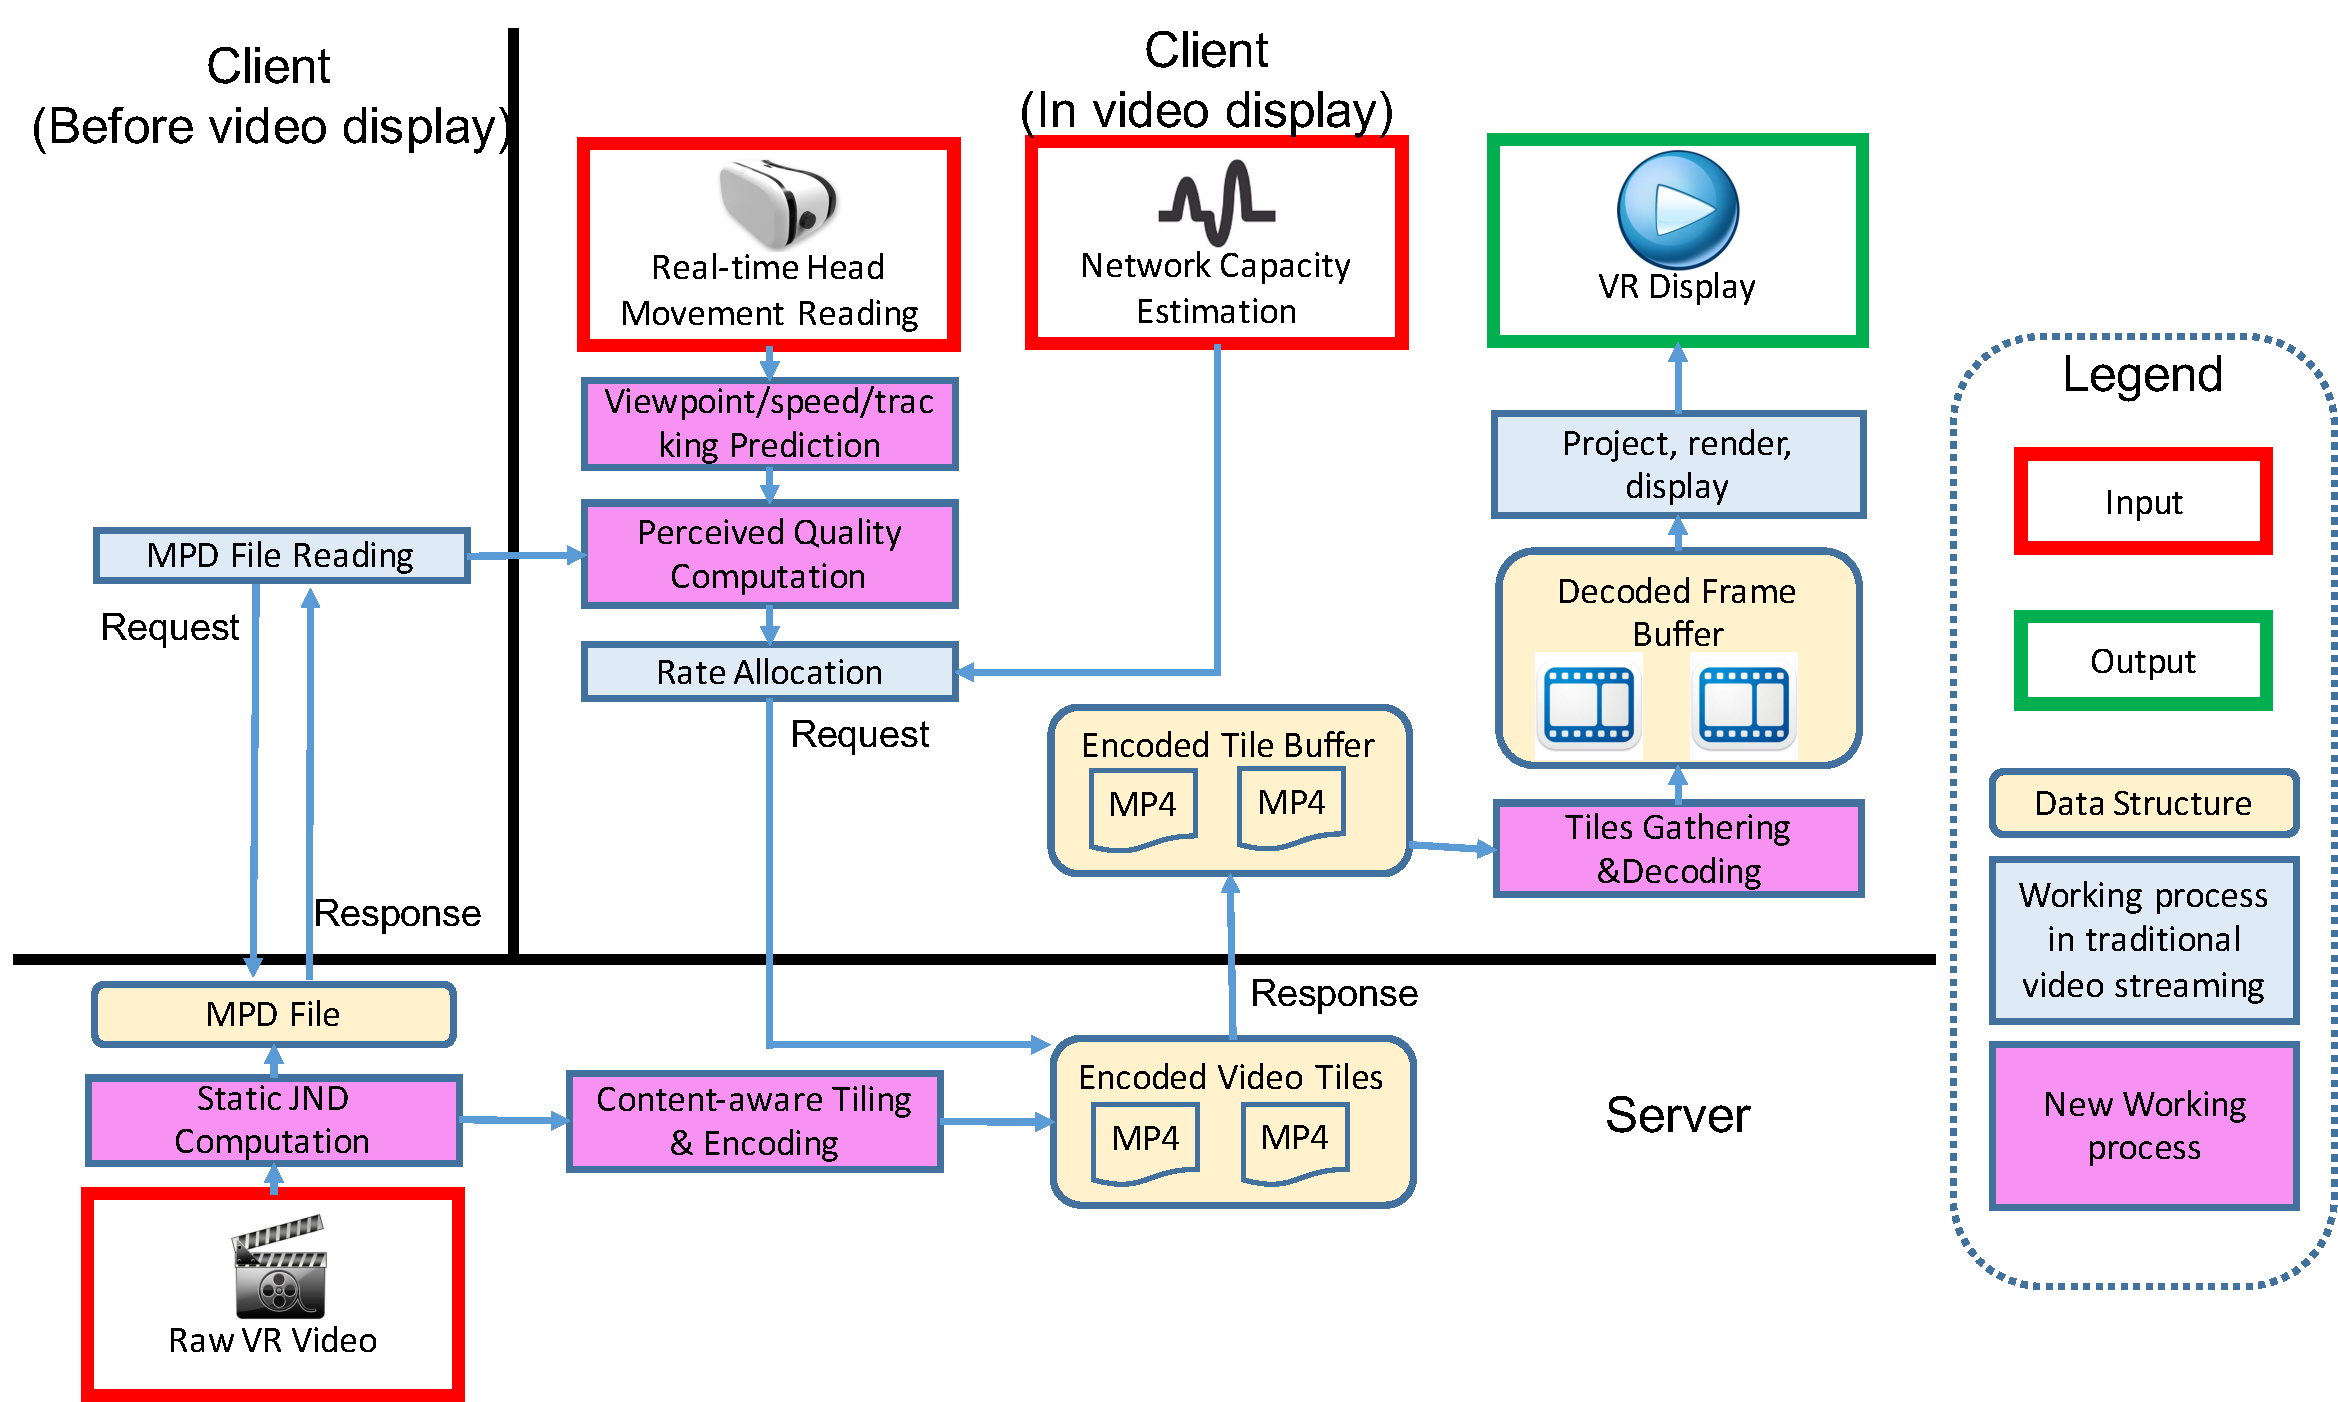
\includegraphics[width=3.5in]{images/implementation.pdf}
  \caption{Workflow of PQVRS.}
  \label{implementation}
  \end{figure}

Implementation of PQVRS is shown in Fig. \ref{implementation}. Compared with traditional video streaming system, several modules are newly added or modified, which are highlighted by pink color.

\subsubsection{Server-Side}

\textbf{Static JND Computation:}

\textbf{Content-Award Tiling / Encoding:}

\subsubsection{Client-Side}

\textbf{Viewpoint / Speed / Tracking prediction:} In our system, viewpoint prediction is achieved by linear regression because of its efficiency and robustness. According to result of viewpoint prediction, we can estimate user's viewpoint moving speed by differentiating adjacent user viewpoints. Moreover, since we have analyzed object traces of video on server-side and deliver the brief description to client-side, client-side can match the predictive viewpoint traces and object traces in order to predict if user is going to tracking an object.

\textbf{Perceived Quality Computation:}

\textbf{Tiles Gathering \& Decoding:}

\subsection{Challenges in an operational setting}

